\documentclass{article}

\usepackage{amsmath}
\usepackage{verbatim}
\usepackage[margin=0.75in]{geometry}
\usepackage{graphicx}
\usepackage{float}
% usepackage{algorithm2e}

\title{ABM project - Glosten Milgrom Model}
\author{Yu-Kuan Lin (K21030132), Atanasije Lalkov (K21108925),\\
Mohit Narayan Shah (K21041514), Ying-Jui Chu (K21062543)}
\date{}  % Do not show date

\begin{document}
\maketitle

\graphicspath{ {./images/} }

\section{Abstract}
This report builds on the sequential information model, Glosten Milgrom Model, proposed in 1985\cite{gm:1985}. We start by introducing the Glosten Milgrom Model, and then we discuss the variations we made to the model to explore different scenarios and their consequent results. In particular, we perform sensitivity analysis on the proportion of informed traders in the trader population, we test whether having the correct initial guess of bullish/bearish market matters a lot for the market maker's learning process, we let uninformed traders be inactive from time to time, and we introduce partially informed traders to generalise the amount of information possessed among the trader population.

\section{Introduction}
Glosten Milgrom model is a simulation model designed to portrait the process of which information impacts the formation of transaction price in a market-maker market. The process can also be thought of how a market-maker market arrives at its price equilibrium driven by information under the competitive market settings. In particular, the key of this process is the market maker learning the fundamental value of the traded security in order to make her quotes. In this section, we introduce our implementation of the original Glosten Milgrom Model, and we also discuss briefly what other the experiments we have carried out by extending the original model.

\subsection{Glosten Milgrom Model}\label{GM Model}
In a market-maker market, the traders come to the market maker with their orders (either buying or selling). The market maker now has to determine her\footnote{In this report, we refer to the market maker as female and to the traders as males. This practice is suggested by Osborne. See the preface in reference \cite{gametheory:1994}.} quotes. Let $V$ be the fundamental value of the traded security, which is unknown to the market maker. The rational thing to do here is to make her quotes according to the value of $V$ because her profit depends on it. In particular, under competitive market settings, her best policy is to make quotes such that her profit per transaction is zero. Since the value of $V$ is unknown to the market maker, the challenge for her is to learn the value of $V$ in order to make quotes accordingly. We thus have formula \ref{math:profit per buy order} and \ref{math:profit per sell order}.
\begin{equation}
    E(\text{profit}|\text{buy order}) = E(\text{bid} - V|\text{buy order}) = \text{bid} - E(V|\text{buy order}) = 0
    \implies \text{bid} = E(V|\text{buy order})
    \label{math:profit per buy order}
\end{equation}
\begin{equation}
    E(\text{profit}|\text{sell order}) = E(V - \text{ask}|\text{sell order}) = E(V|\text{sell order}) - \text{ask} = 0
    \implies \text{ask} = E(V|\text{sell order})
    \label{math:profit per sell order}
\end{equation}

In Glosten Milgrom Model, the value $V \in \{V_L, V_H\}$ is set to follow a bernoulli distribution with $p(V = V_L) = \sigma$. The meaning behind this setting is that the value of the traded security can either go low (denoted by $V_L$) or high (denoted by $V_H$), with the probability of going low being $\sigma \times 100\%$. Hence the functions for making quotes now become\footnotemark{}:
\begin{equation}
    \text{bid} = E(V|\text{buy order}) = \sum_{i \in I}{p(V_i|\text{buy order})V_i} = \sum_{i \in I}{\frac{p(\text{buy order}|V_i)p(V_i)}{p(\text{buy order})}V_i}, \quad I = \{H, L\}
\end{equation}
\begin{equation}
    \text{ask} = E(V|\text{sell order}) = \sum_{i \in I}{p(V_i|\text{sell order})V_i} = \sum_{i \in I}{\frac{p(\text{sell order}|V_i)p(V_i)}{p(\text{sell order})}V_i}, \quad I = \{H, L\}
\end{equation}
\footnotetext{Note that we applied Bayesian formula to arrive at the final form of the functions. This demonstrates the "Bayesian learning nature" of making quotes according to information. Also, in pratice, $p(\text{buy order})$ is computed as $\sum_{i \in I}{p(\text{buy order}|V_i)p(V_i)}$, and similarly, $p(\text{sell order}) = \sum_{i \in I}{p(\text{sell order}|V_i)p(V_i)}$.}

To explain how the model works, let's see who are the agents within the market (environment). There are three types of agents in the market: informed traders (denoted by $I$), uninformed traders (denoted by $U$), and a market maker (denoted by $M$). The traded security $V$ can have a fundamental value of low or high (denoted by $V_L$, $V_H$), and only the informed traders $I$ have the information of whether $V$ equals to $V_L$ or $V_H$. Assuming the traders act rationally, we can address their strategies as following:

\begin{itemize}
    \item The informed traders will submit a sell order if $V$ equals to $V_L$ and buy order if $V$ equals to $V_H$.
    \item The uninformed traders do not have any information, so they will submit a buy order with probability $\gamma$. (With zero information, we set $\gamma$ to $0.5$ to reflect the highest entropy.\footnotemark{})
\end{itemize}
\footnotetext{We consider an extreme case of asymmetric information in the market, i.e., the uninformed traders have no information at all.}

At the beginning of a simulation, we sample the fundamental value $V$ from a bernoulli distribution. We then set up a trader population with $\mu \times 100\%$ informed traders and $(1-\mu) \times 100\%$ uninformed traders. For every iteration, a trader is randomly picked from the trader population. He submits an order to the market maker according to his strategy. The transaction is then executed after $M$ offers her quotes. As orders keep arriving, the market maker gradually learns the true value of $V$ with Bayesian learning and improves her quotes accordingly. In our implementation, we then halt the simulation when the learning process has converged\footnotemark{}. We list some remarks regarding the assumptions and settings of the implementation of the original Glosten Milgrom Model.

\footnotetext{In our implementation, we perform Cauchy convergence test to check whether the learning process has converged. In particular, we store the value of $M$'s confidence level of her estimation of $V$ being $V_L$ as the learning process progresses. The Cauchy convergence test is performed on the sequence of the confidence levels.}

\begin{itemize}
    \item Inventory is not an issue for the market maker, hence every order is executed right away.
    \item Only one security is traded in the market.
    \item Fundamental value $V \in \{V_L, V_H\}$ follows a bernoulli distribution with a constant parameter $\sigma$ denoting the probability of $V=V_L$.
    \item Tradable size of the security is fixed to one unit.
    \item Under competitive market settings, M chooses to play her best strategy - makes quotes such that her expected profit is zero.
    \item $M$ knows everything about $\sigma$ (probability of $V = V_L$), $\mu$ (fraction of $I$ in the trader population), and $\gamma$ (probability of $U$ buying).
    \item $M$ cannot distinguish between informed and uninformed traders.
    \item The traders are always active, i.e., upon being chosen, they always submit an order.
    \item There only exists fully informed and fully uninformed traders.
\end{itemize}

\subsection{Our experiments}\label{Our Experiments}
Regarding our experiments with the original Glosten Milgrom Model, we take advantage of programming in Python to provide flexibility, scalability, computation efficiency, and ease of manipulation/analyses for our implementation. We start by analysing some of the model parameters, and then we create two different variants of the model to explore different scenarios. In the meantime, we montior the efficiency\footnote{The efficiency is measured by how many orders the market maker needs to learn the true value of $V$.} of the learning process of $M$ and the distribution of cumulative profit and loss\footnotemark{} among the agents (traders and the market maker). To elaborate, here are our experiments that will be addressed in the upcoming sections:

\footnotetext{The cumulative P\&L measures the profit and loss of the players after going through $M$'s learning process. The distribution of the cumulative P\&L among the players measures the allocation of wealth among the agents after the process.}

\begin{itemize}
    \item In section \ref{sigma and mu}, we explore different levels of $\sigma$ (probability of $V$ being $V_L$) and $\mu$ (proportion of fully informed traders) and their impact to convergence and P\&L allocation. The implication of different levels of $\sigma$ is the market condition being bearish or bullish in various degrees, while $\mu$ controls how many informed traders are there in the trader population.
    \item In section \ref{inactive U}, we give the uninformed traders opportunity to refrain from trading. The reasoning of this alteration is that due to the lack of information, $U$ have less incentive to trade frequently in comparison to $I$. This implementation results to $M$ sometime not receiving any orders (buy/sell orders).
    \item In section \ref{P trader}, we introduce a new type of trader to the market - partially informed traders $P$. Unlike fully informed traders $I$, partially informed traders do not always act based to the information. In other words, they are not completely confident about the information they have, resulting in the possibiliy of them submitting orders in the wrong direction. This generalises the model in which traders can have distinct level of confidence in the information they possess.
\end{itemize}

\section{Initial belief and sensitivity of $\mu$}\label{sigma and mu}
During trading, the market maker tries to ensure that the quotes she provides result in her profit being equal to zero on average, which is a strategy for a market maker in a competitive market that results in a equilibrium. The prices (asks and bids) are set by the market maker depending on the type of order the trader submits. For the market maker to provide a quote, requires the use of Bayesian inference to update her estimation of $V$. Before any orders are received from the traders, the market maker has a prior belief in the traded security used to determine the market maker's quote. Is it important for $M$ to have an accurate initial guess ? 

\subsection{Impact of initial belief to market maker's Bayesian learning}
Before the market maker receives any orders, how much information does the market maker have to make assumptions about her initial estimation ? She initially has no information regarding the value of the asset therefore the entropy is high as there is no information, thus her initial belief would be 0.5 (equal chance of $V=V_H$ or $V=V_L$) making it highly uncertain. This is the assumption made when observing the agent-based model's normal behaviour.

Within actual markets, does the market maker have no information regarding her environment (the market)? We can then instead assume that the market maker has some information about the current market trends whether it is a bullish or bearish market, as within markets all agents still have basic access to information. As we increase the market maker's information set we will be able to model her beliefs in different market conditions. Therefore, if the market has bullish views of the market she can update her initial belief of $V$, and vice versa if the market view is bearish. The agent (market maker) has now decreased the entropy and we will model this to observe her learning efficiency.

Modelling the market maker's initial beliefs in different environments requires setting the environment to a bullish market which is done by decreasing the value of parameter $\sigma$ which increases the probability of $V_H$ being the value of the asset. Also, update the market maker's initial belief of the market being bullish. We model the different conditions which include the normal behaviour of the model, a bullish market where the market maker has bullish assumptions of the trend and finally a bearish market where the market maker still has a bullish assumption of the market. By simulating the agent-based model multiple times\footnote{For a market condition we have a sample size of 100 iterations } under the different market conditions, we can observe the results below in table \ref{tlb:normal conditions}, showing the market maker's efficiency, which is the average number of orders required for the market maker to update her belief of the asset value until that it converges to the true value of the asset. For each market condition, multiple iterations are simulated to obtain a mean learning efficiency. Observing the different environments of the market we can establish that the learning efficiency does not change significantly. 

\begin{table}[ht]
    \centering
    \begin{tabular}{ |p{3cm}||p{3cm}|p{3cm}|p{3cm}|  }
        \hline
        \multicolumn{4}{|c|}{$M$'s initial belief: bullish market} \\
        \hline
        Market type& Initial belief & $\sigma$ & Learning efficiency\\
        \hline
        Normal & 0.5 & 0.5 & 49.02\\
        Bullish& 0.4 & 0.25& 50.31\\
        Bearish& 0.4 & 0.75& 49.08\\
        \hline
       \end{tabular}
       \caption{Learning efficiency in mildly bullish/bearish conditions}
       \label{tlb:normal conditions}
\end{table}

We can analyse the sensitivity by increasing the difference between the market maker belief and the actual market trend. We update the environment by setting stronger bullish and bearish trends, whilst the market maker's belief stays constant (table \ref{tlb:extreme conditions}). We can observe the results by simulating the agent-based model which indicates no change to the market maker's efficiency when we imply a stronger trend in the environment as shown in table \ref{tlb:extreme conditions}. 

\begin{table}[ht]
    \centering
    \begin{tabular}{ |p{3cm}||p{3cm}|p{3cm}|p{3cm}|  }
        \hline
        \multicolumn{4}{|c|}{$M$'s initial belief: bullish market} \\
        \hline
        Market type& Initial belief & $\sigma$ & Learning efficiency\\
        \hline
        Normal & 0.5 & 0.5 & 48.71\\
        Bullish& 0.4 & 0.1 & 49.56\\
        Bearish& 0.4 & 0.9 & 51.51\\
        \hline
    \end{tabular}
    \caption{Learning efficiency in extreme bullish/bearish conditions}
    \label{tlb:extreme conditions}
\end{table}

 This shows the robustness of the initial belief, which states that the initial belief of the market maker is not that important to her learning as we obtain the same efficiency no matter what initial belief the market maker has in different types of market environments. Intuitively we anticipated that having closer initial belief to the actual market condition would result in a better learning efficiency, however the robustness of the initial belief indicates that it does not matter for this type of learning process.

\subsection{The sensitivity of $\mu$}
A key factor of the market maker's learning process is the parameter $\mu$ (fraction of informed traders in the trader population). By varying $\mu$, how will it affect the market maker's learning of the asset value? Supposedly our first assumption is that with greater presence of informed traders in the market, there is much more information coming from the orders, leading to a more effortless learning process for $M$.

To observe the market makers learning efficiency requires observing the number of orders needed for the market maker to update her belief of asset value so that it converges to the asset's true value, with parameter $\mu$ varying. By varying $\mu$ within the interval $[0,1)$, we obtain the following observations in figure \ref{fig:mu}, where we can observe the number of orders required by the market maker to learn and the x-axis shows the fraction of informed traders in the market. 
Analysing the simulation results in figure \ref{fig:mu} shows that for low values of $\mu$ (less informed traders in the marker) the market maker does not learn the true value of the asset. When $\mu$ increases the market maker starts to learn, and we can observe a trend when the market maker does learn, which is as $\mu$ increases the efficiency increases. Overall, due to informed traders knowing the true value of the asset, it will ultimately mean the market maker's belief is not distorted by the noise of uninformed traders so each time an order is received significantly improves her belief of the asset value. In terms of sensitivity analysis, this indicates high levels of sensitivity as a change of $\mu$ from 0.18 to 0.3 results in a large change from the market maker not learning to the market maker learning in 50 orders.

\begin{figure}[h]
    \centering
    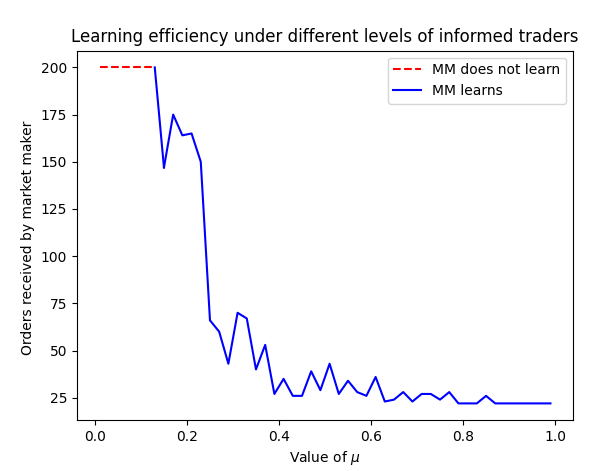
\includegraphics[scale=0.6]{mu.png}
    \caption{Learning efficiency under different levels of informed traders}
    \label{fig:mu}
\end{figure}

\subsection{Welfare among agents: varying $\mu$}\label{Welfare}
A key aspect of agent-based modelling is observing the welfare of the agents and within this model, it is the welfare of the: informed traders, uninformed traders and the market maker. To measure the welfare in a market can be done in multiple ways but for this model, the welfare will be the profit made by each agent throughout the learning process of $M$. We monitor the distribution of welfare among the agents with different underlying $\mu$.

Simulating the agent-based model we obtain the simulation results in figure \ref{fig:pnl distribution}. The results show the welfare distribution of each agent when $\mu  \in \{0.2,0.5,0.8\}$. For each value of $\mu$ we iterate 1000 times to come up with a distribution of cumulative welfare among the agents.   

The standard deviation decreases as $\mu$ increases. We can infer that the effectiveness of the agent predicting their P\&L is positively correlated to the level of $\mu$.Informed traders always have positive welfare compared to the other agents, which is the result of exploiting asymmetric information in the market. Uninformed traders mostly have negative welfare as they are inferior compared to the other agents. Whilst market maker's welfare varies a lot due to the varying degree of information she posses. 

\begin{figure}[ht]
    \centering
    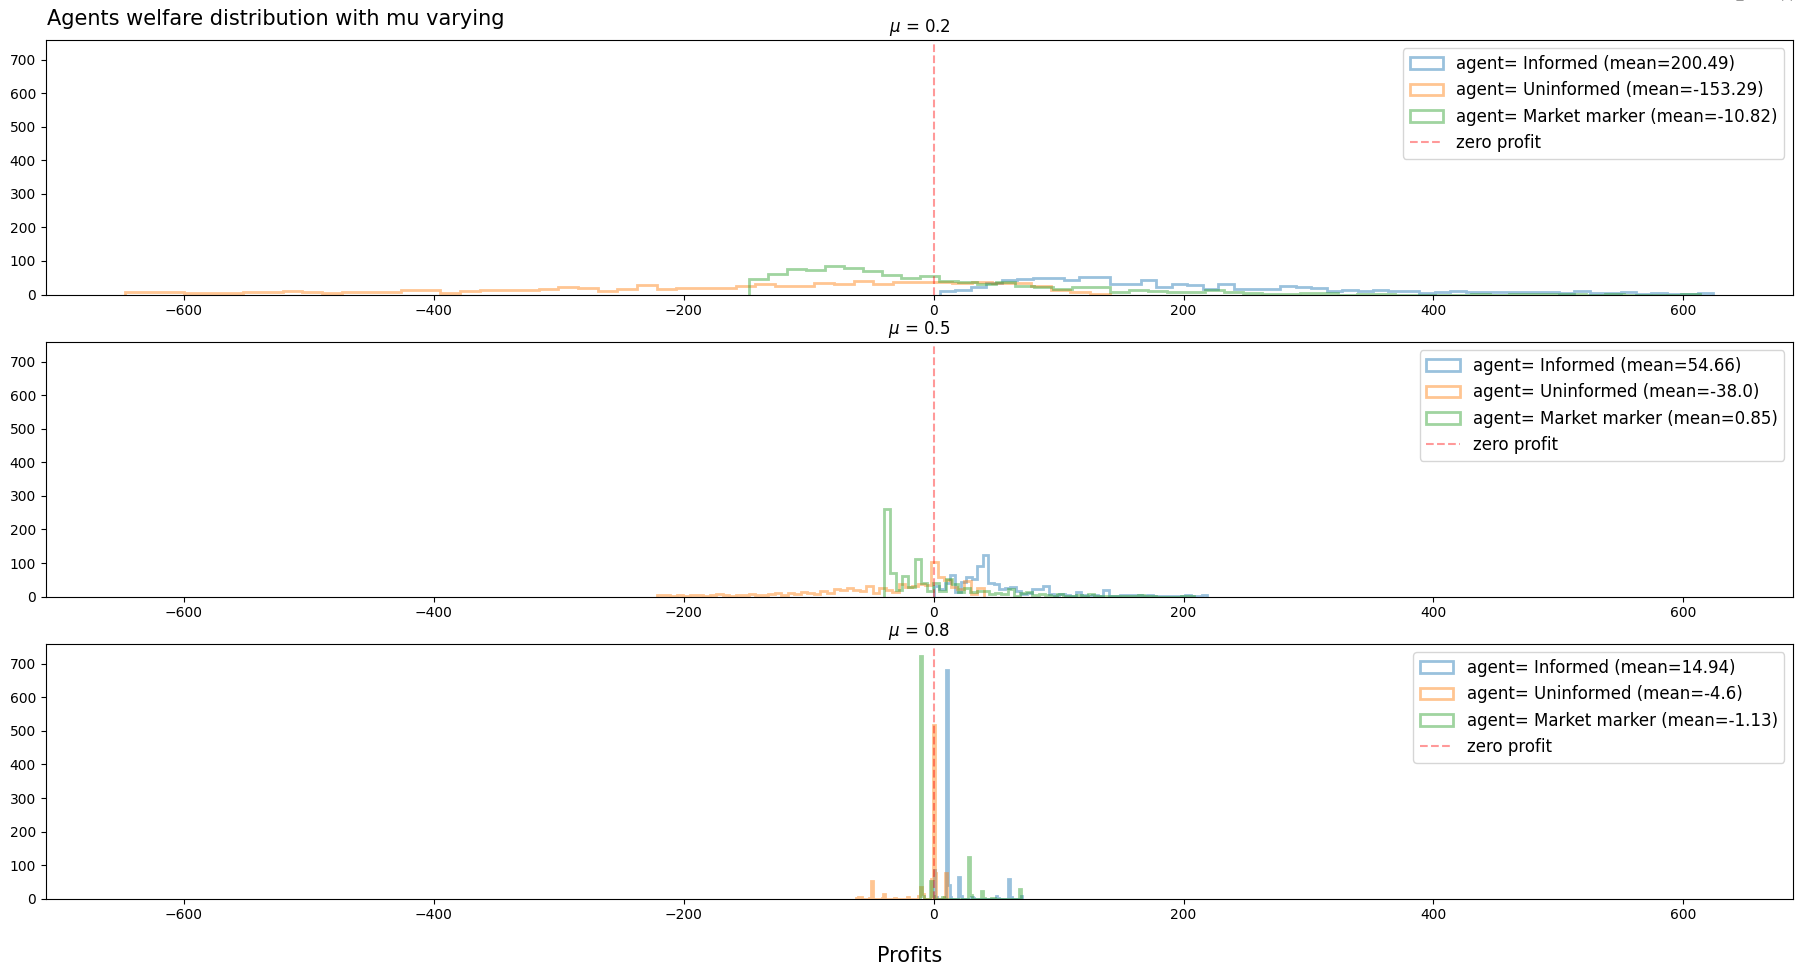
\includegraphics[width=17cm,height=10cm]{welfare.png}
    \caption{Distribution of cumulative profit and loss}
    \label{fig:pnl distribution}
\end{figure}

\section{Introducing inactive uninformed trader}\label{inactive U}
In the original Glosten Milgrom Model, the market maker follows a process of gathering information from the orders submitted by the traders in a sequential manner. Also, in this model there are two types of traders: informed traders and, uninformed traders. We refer to the traders being active as they always submit orders. The informed traders in this model submit orders based on some valid information that they have about the market, while the uninformed traders make trades based on no information. So, they are basically incorporating noise in the information gathering process.

Now, we add another feature to the uninformed trader in this model according to which the uninformed traders can choose to remain inactive (not making a trade). Instead of always submitting an order randomly without any information, we now introduce a new probabilistic parameter called $\theta \in [0,1]$ that controls the probability of uninformed trader remaining active in our model. This implies that when $\theta = 1$ then uninformed trader will always submit an order randomly, while $\theta = 0$ implies uninformed trader will always remain inactive i.e., does not submit an order. Let's observe the role of $\theta$ in the market.

\subsection{Varying proportion of inactive uninformed traders}
When $\theta$ is high, uninformed traders will make random trades more often. So, this means that the proportion of noise in the information is at it's highest, implying the learning process will be slow because the density of information will be low. In contrast, when $\theta$ is low, more often than not uninformed traders will remain inactive because of which market maker will have a higher density of information as the higher proportion of orders will come from informed traders. So, we can conclude that the lower the number of orders coming from the uninformed traders, lower will be the noise in the market and hence the market maker converges her learning process more quickly in predicting the true value of the asset.

In the figure \ref{fig:v2_efficiency_theta} below, we perform 50 simulations for each $\theta$ and configure a box plot from which we can observe that the value of $\theta$ is directly proportional to the number of order it requires for the market maker's estimation to converge to the true value of the asset. In other words, the learning efficiency is inversely proportional to the value of theta.

Another observation we can arrive at is the increasing trend of volatility with respect to the number of orders it takes M to estimate the true value of the asset with increasing $\theta$. Elaborating on the previous point, lower efficiency implies more room for noise, resulting in more volatile learning process.

\begin{figure}[h]
    \centering
    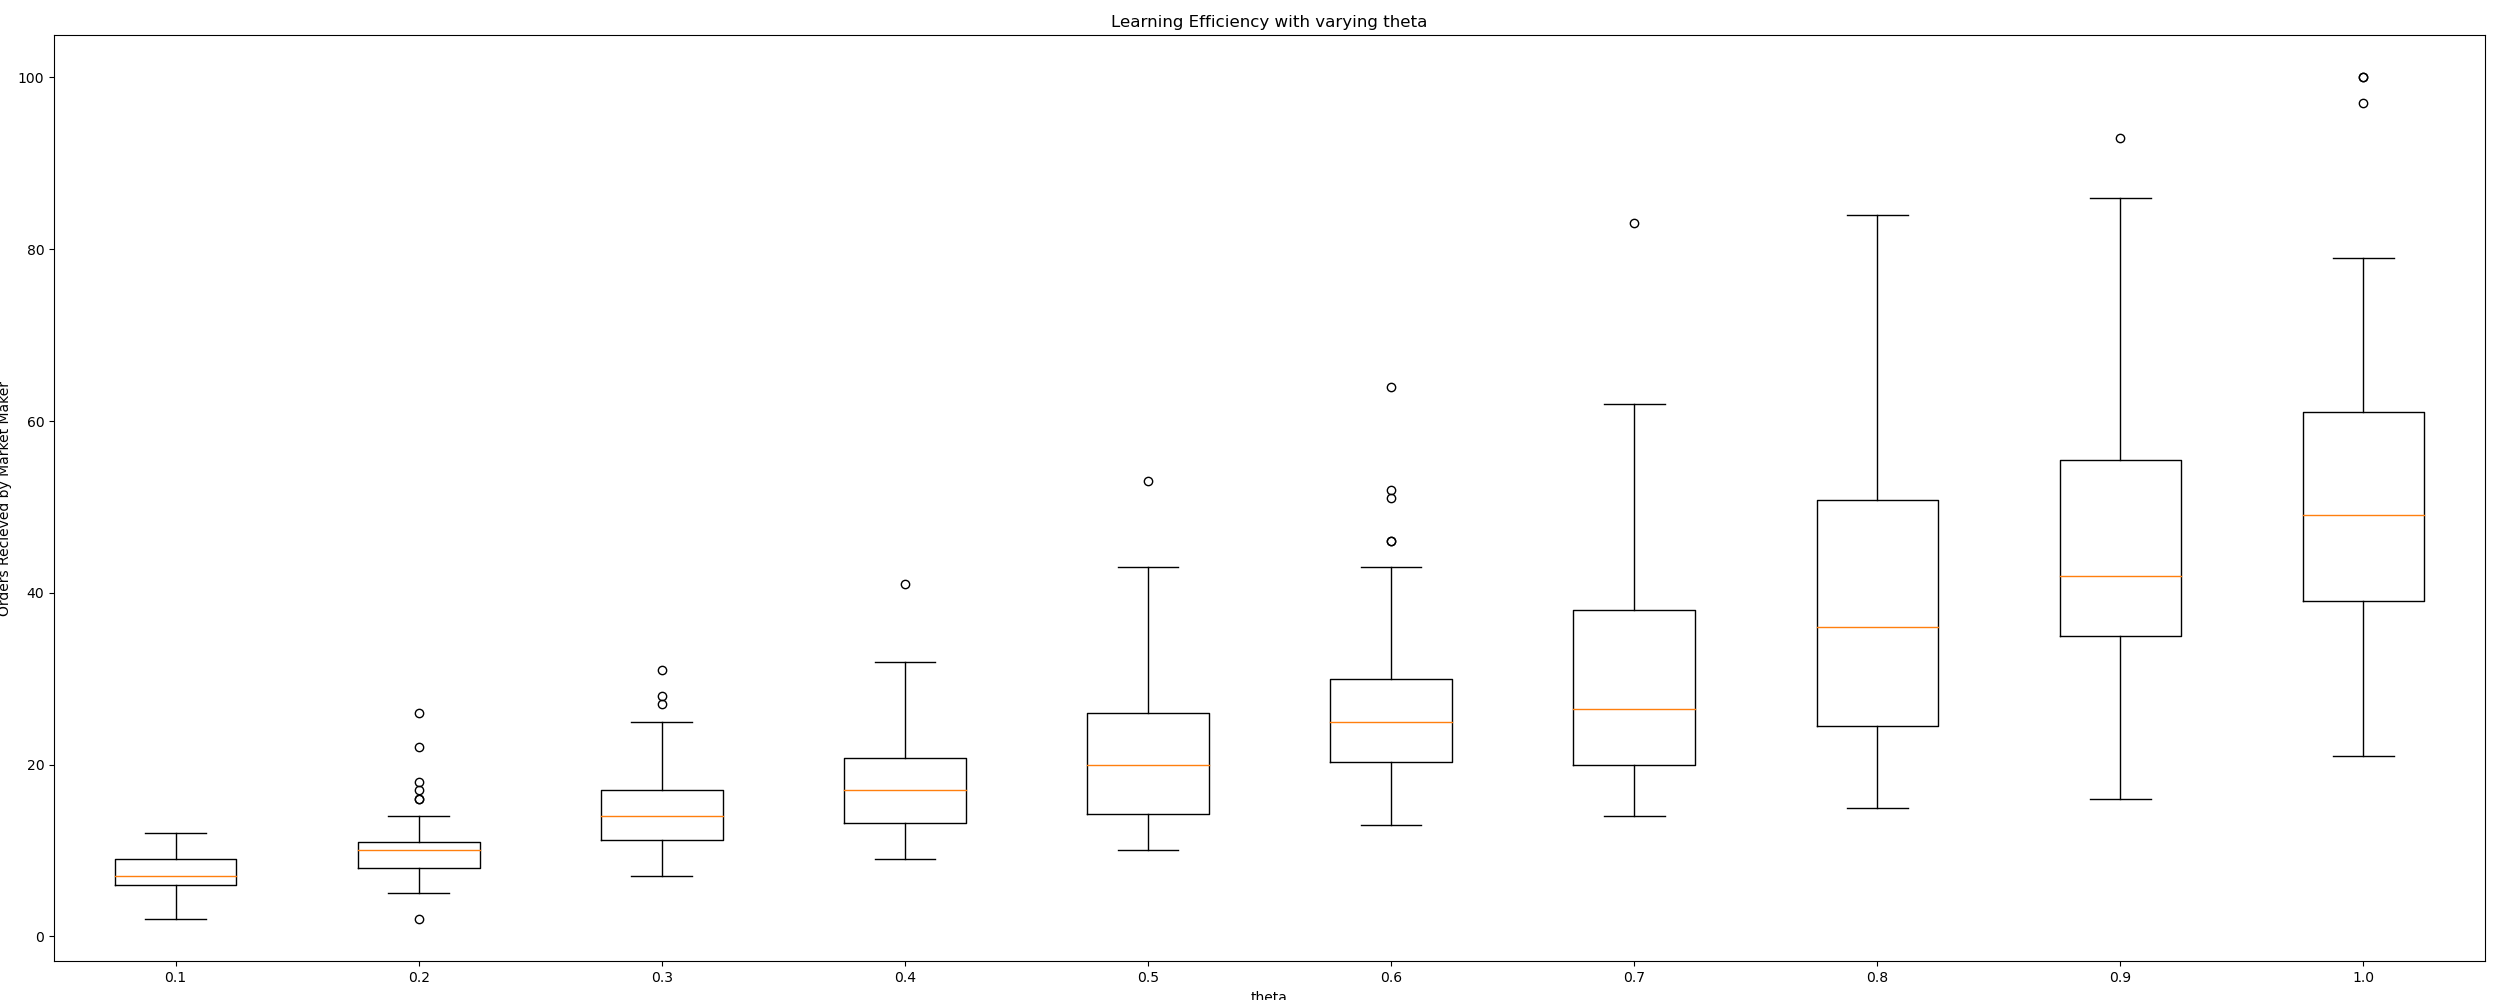
\includegraphics[scale=0.28]{v2_efficiency_theta.png}
    \caption{Learning efficiency under varying $\theta$}
    \label{fig:v2_efficiency_theta}
\end{figure}

\subsection{Perspective of liquidity with varying $\theta$}
Continuing with the analysis of $\theta$, we will now observe the liquidity. In terms of liquidity in our model, seeing that all submitted orders are executed, translates to a higher liquidity with the increase in the number of submitted orders. If $\theta$ decreases, the number of submitted orders decreases, causing lower liquidity. So, we can infer that $\theta$ drives liquidity in this market. However, all this is conditional on the second factor $\mu$ ,which would be able to compensate for $\theta$, i.e., increasing $\mu$ can compensate for decreasing $\theta$ with respect to liquidity.

\subsection{Welfare among agents: varying $\theta$}
We vary $\theta$ and monitor the welfare of the agents as done in section \ref{Welfare}. Now, we simulate the Agent based model for 1000 iterations for each $\theta \in \{0.2, 0.6, 0.9\}$. Observing the simulation results in figure \ref{fig:v2_welfare_theta} below, we notice a trend that the variance of the agent's welfare is positively correlated to $\theta$. With decreasing $\theta$, the agents are more certain about their welfare, which explains the low variance within the histograms. This whole observation makes sense because trading is a zero sum game between the market maker and the traders.

\begin{figure}[H]
    \centering
    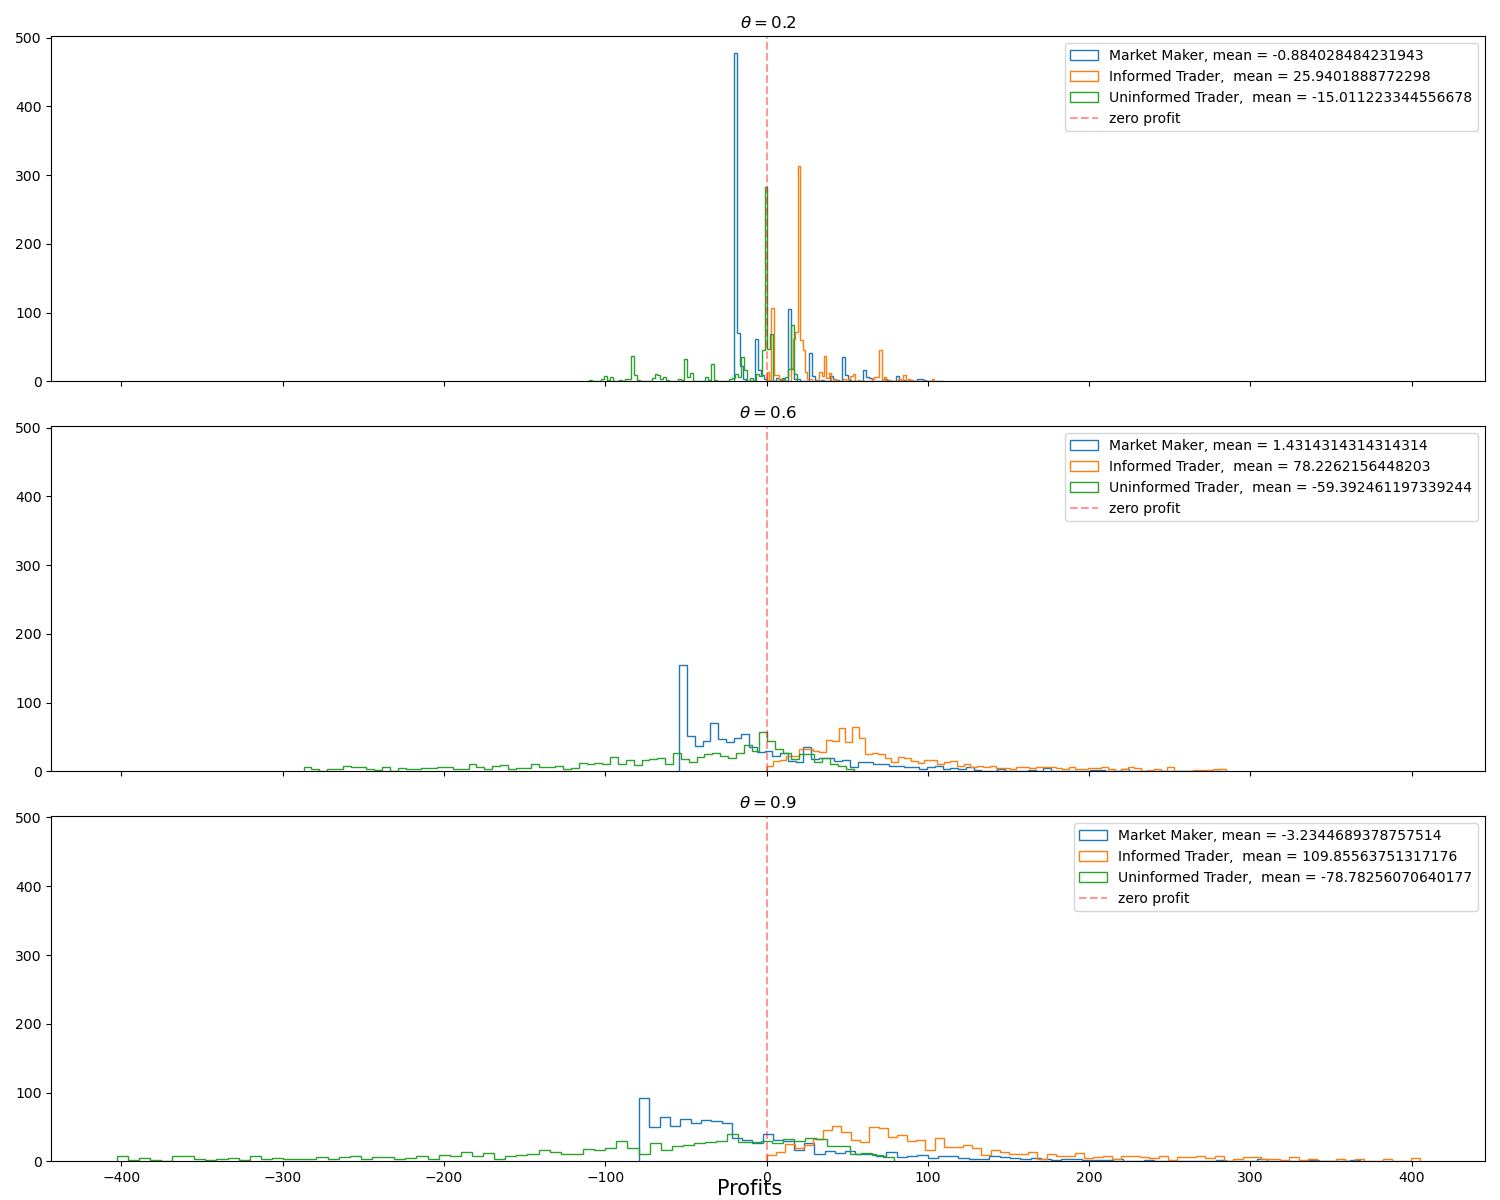
\includegraphics[scale=0.45]{v2_welfare_theta.png}
    \caption{Welfare of Agents under varying $\theta$}
    \label{fig:v2_welfare_theta}
\end{figure}

\section{Partially informed trader}\label{P trader}
We change $\mu$ to $\mu_i$ denoting the proportion of fully informed trader and introduce a new agent, partially informed trader $P$, also two parameters, $\mu_p$ and $\eta$, to the fundamental Glosten Milgrom model. $\mu_p$ denotes the fraction of partially informed trader ($P$) and $\eta \in [0, 1]$ represents the confidence level that partially informed traders submit their orders in the correct direction. This section focuses on how $P$ interacts with other agents also addresses the relationship between $\eta$ and the agents in the market. 

Under the given premises, for $\eta \in [0, 0.5)$, $P$ mostly submit orders in the wrong direction, which we define as an irrational action. For $\eta \in (0.5, 1]$, $P$ usually submit orders in the correct direction. For instance, $\eta=0.95$ means that 95\% of $P$'s actions are rational, which provides the market maker correct information most of the times; $\eta=0.05$ indicates that only 5\% of $P$'s actions are rational, with 95\% of the information being deceiving for $M$.

\subsection{Learning efficiency with varying $\eta$}
We start by withdrawing $I$ from the market then observe how $\eta$ and $\mu_p$ affect the market. Figure \ref{fig:large eta} and Figure \ref{fig:small eta} have four subplots each with the former one having $\eta \in \{0.5, 0.65, 0.8, 0.95\}$, and the latter one having $\eta \in \{0.05, 0.2, 0.35, 0.5\}$ respectively. Each individual subplot has x-axis denoting $\mu_p$, and y-axis denoting the number of orders to converge the learning process. The observation of $\eta = 0.5$ implies zero information gain for $M$; $P$ do not provide $M$ with valuable information to converge her learning process. On the other hand, $\eta \rightarrow 0$ or $\eta \rightarrow 1$ provides greater information gain, and $M$ is capable of learning faster. Intuitively, $\eta \in (0, 0.5]$, $M$ is not supposed to converge her learning process due to the significant proportion of deceiving information provided to her. Figure \ref{fig:small eta} shows that $M$ is still able to learn from the false information and predict the real value correctly. The reason is that because of $M$'s information set, she knows the setting of parameters and understands who submits orders with wrong information; hence, she can distinguish irrational behaviour.

\begin{figure}[H]
    \centering
    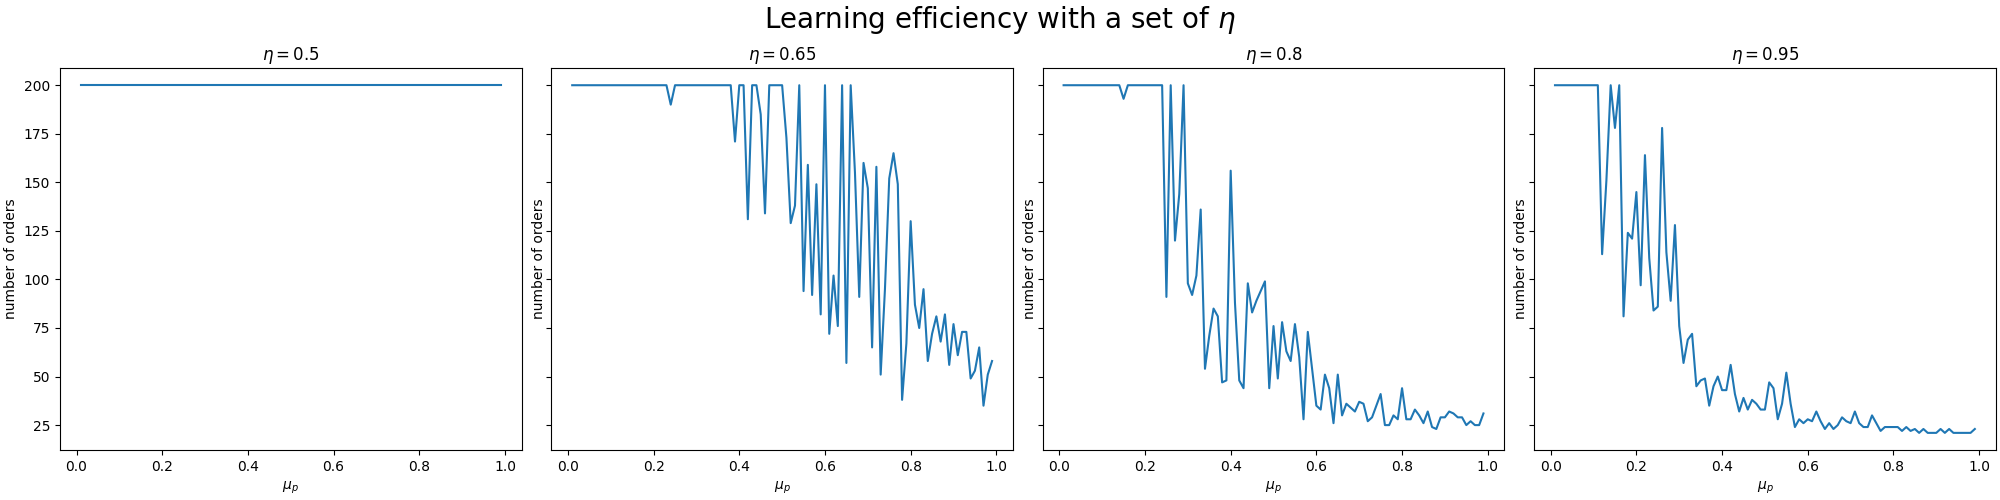
\includegraphics[width=\textwidth]{v3_fig1_large_eta.png}
    \caption{Learning efficiency with large $\eta > 0.5$}
    \label{fig:large eta}
\end{figure}

\begin{figure}[H]
    \centering
    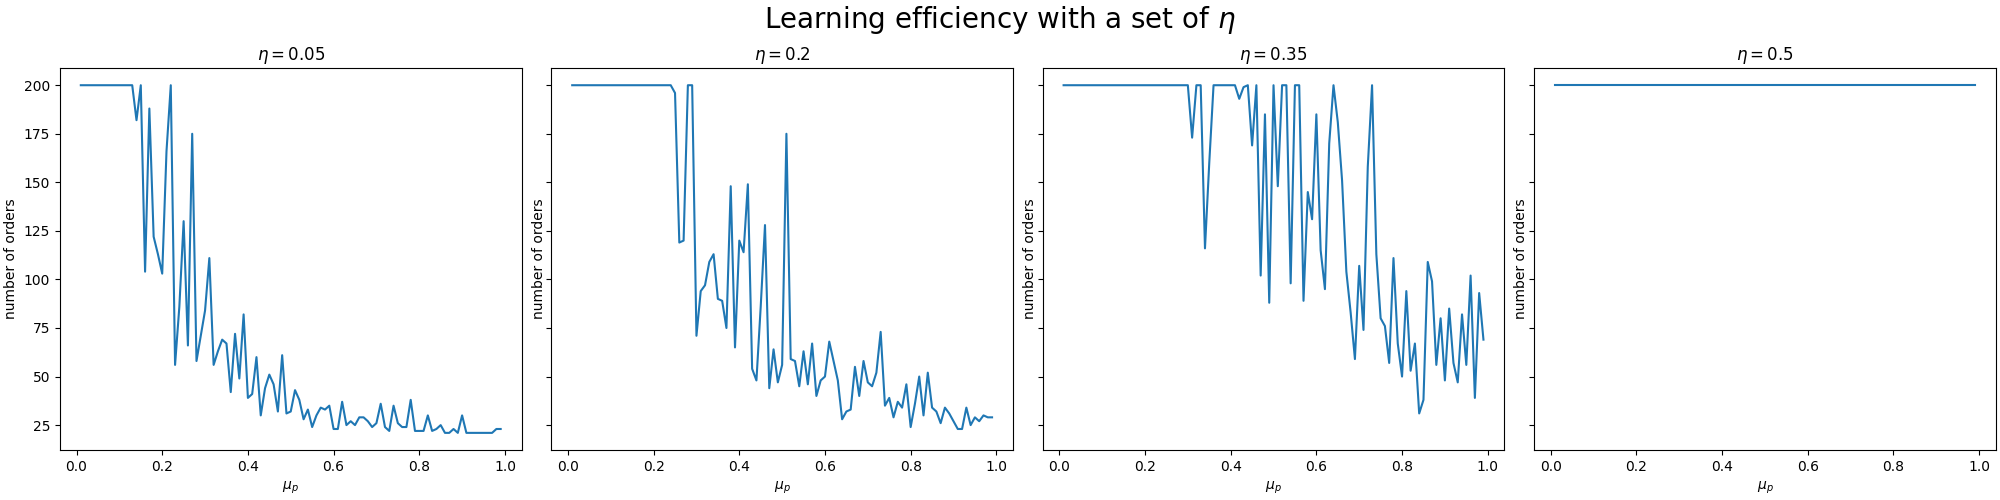
\includegraphics[width=\textwidth]{v3_fig2_small_eta.png}
    \caption{Learning efficiency with $\eta < 0.5$}
    \label{fig:small eta}
\end{figure}

\subsection{Asymmetric results of learning efficiency with varying $\eta$}
Now, we gradually increase the proportion of $I$ in the market and observe the relation between $(\mu_i, \mu_p, \eta)$ and learning efficiency. Figure \ref{fig:fix mu_i} illustrates learning rate heatmaps with $\mu_i \in \{0.1, 0.25, 0.4\}$ in the market. The light blue region represents faster learning speeds; the darker blue represents a lower efficiency of learning; the red indicates learning rate does not yet converge or never converges, and the margin\footnote{The truncated (white) region: no data points in this domain because $\mu_i + \mu_p \leq 1$} represents the proportion of $I$. 

\begin{figure}[ht]
    \centering
    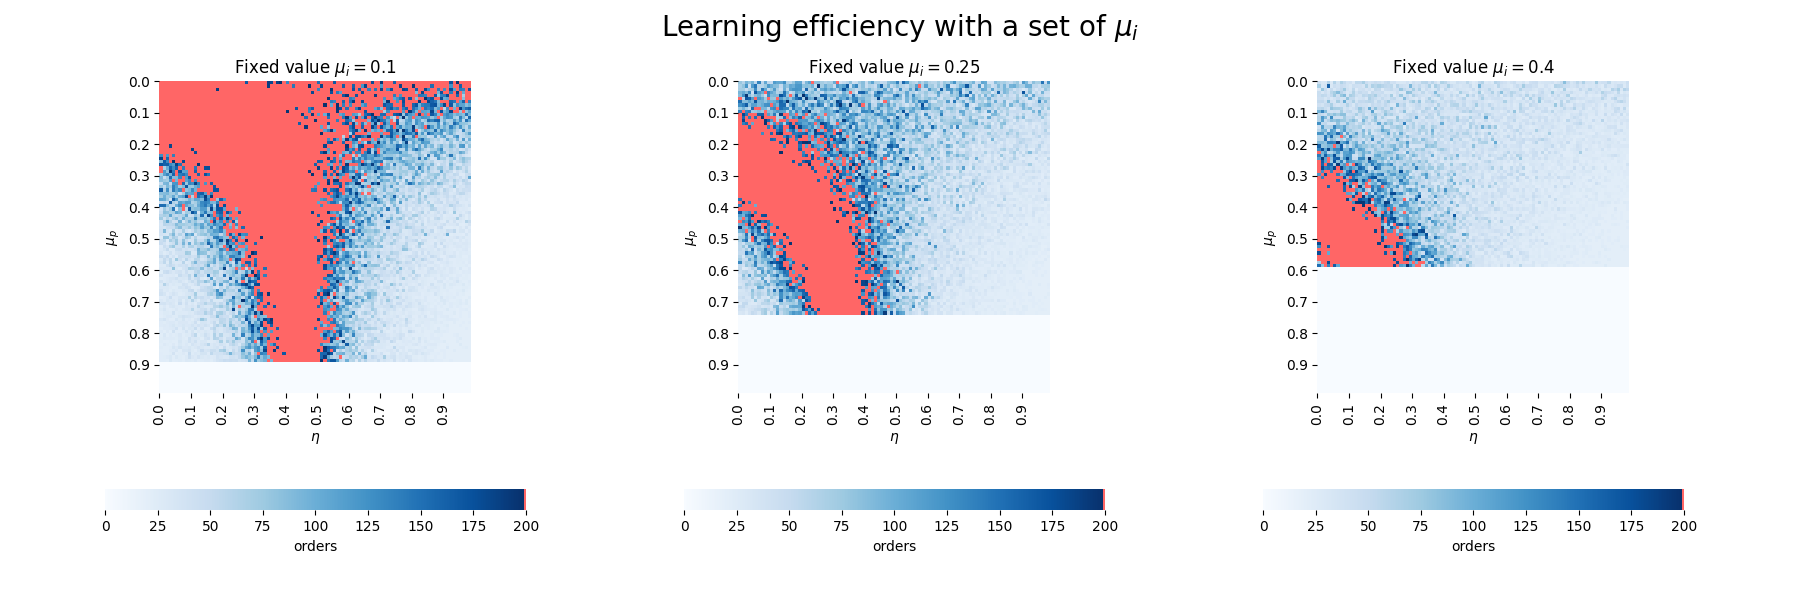
\includegraphics[width=\textwidth]{v3_fig3_heatmap_fixed_mu_i.png}
    \caption{Heatmap of learning efficiency with fixed $\mu_i$}
    \label{fig:fix mu_i}
\end{figure}

From the previous results in figure \ref{fig:large eta} and \ref{fig:small eta}, we expect the heatmap to be symmetric. However, from the results in figure \ref{fig:fix mu_i}, we observe the distribution of red region when $\eta < 0.5$ or $\eta > 0.5$ is asymmetric. When $\eta > 0.5$, most of the information coming from the traders are of the same direction; in contrast, with $\eta < 0.5$, there is a lot of conflicting information leading to more confusion to $M$.

Figure \ref{fig:plot eta} supports the inference we just stated. It shows the percentage of learning process that is unable to converge through varying $\eta$. We found that $M$ starts enhancing her learning efficiency when $\eta$ increases from 0.5; however, for $\eta < 0.5$ shows that a great proportion of simulations of the learning process do not converge. Figure \ref{fig:fix eta_lt} can explain the results when $\eta \in [0, 0.5)$ (Left part of figure \ref{fig:plot eta}). We discover a near equal ratio of correct and deceiving information received from $P$ resulting in $M$ learning process to not converge.

% \newpage
% \vfill

\begin{figure}[ht]
    \centering
    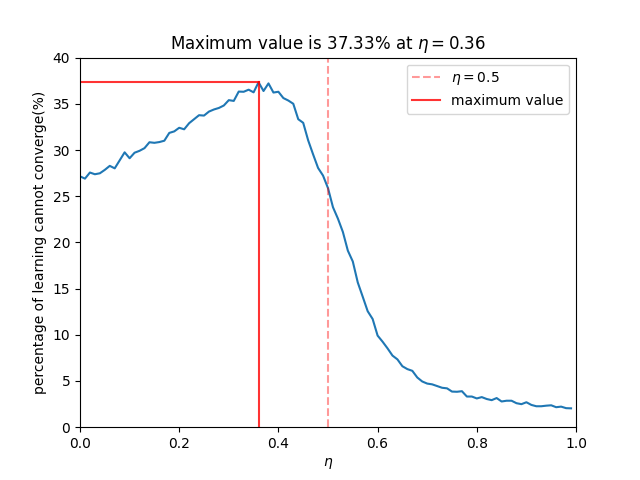
\includegraphics[scale=0.8]{v3_fig9_plot_all_eta.png}
    \caption{Percentage of learning cannot converge}
    \label{fig:plot eta}
\end{figure}

\begin{figure}[ht]
    \centering
    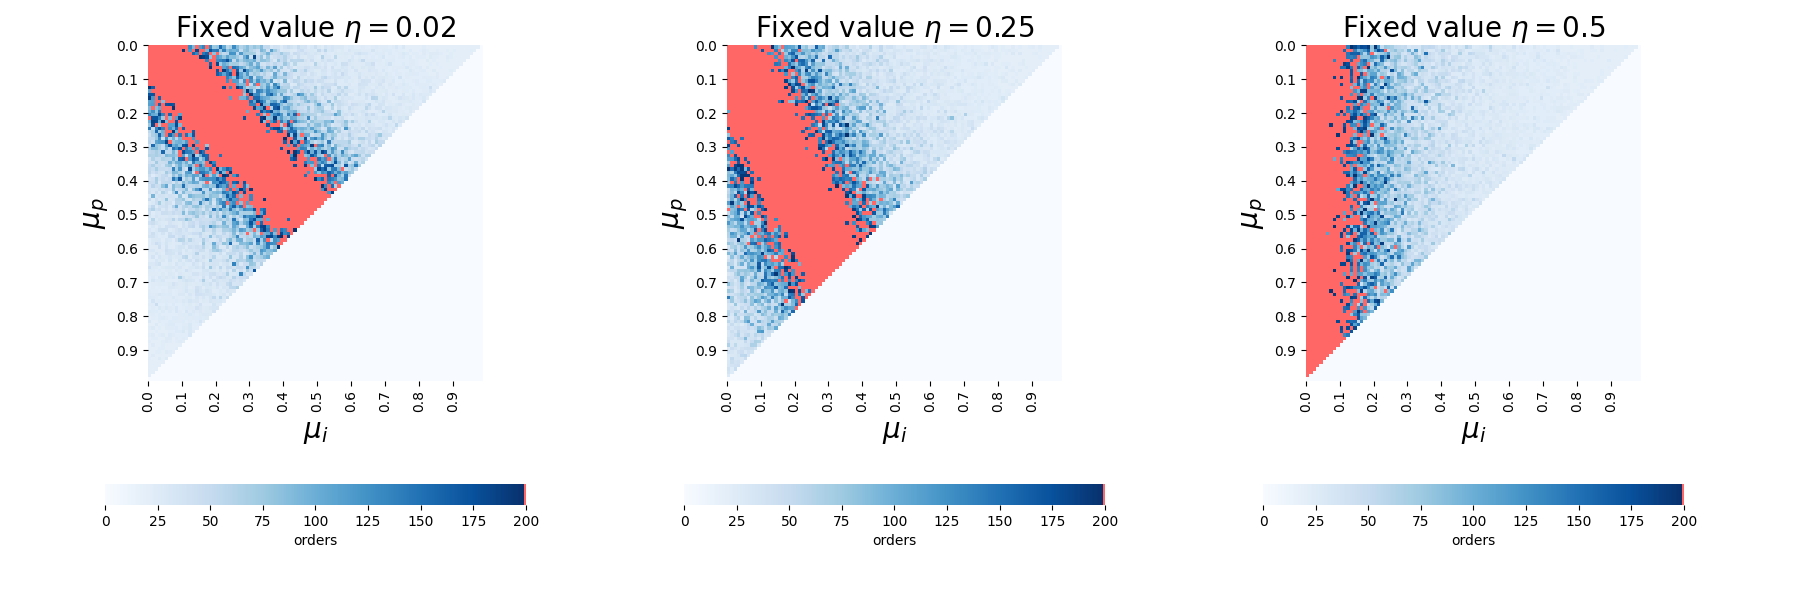
\includegraphics[width=\textwidth]{v3_fig5_heatmap_fixed_eta_lt.png}
    \caption{Heatmap of learning efficiency with fixed $\eta$ ($\eta<0.5$)}
    \label{fig:fix eta_lt}
\end{figure}

% \vfill
% \clearpage

\section{Conclusion}\label{conclusion}
To conclude, we set out to explore the Glosten Milgrom model from an agent-based modelling perspective through analyses of model parameters, introduction of a new strategy, and a new agent to the environment. We have successfully drew insights from different implementations and came up with the explanations for these discoveries. Interestingly, one of our discoveries is that empirical results might not always reflect our intuitive believes. That is one of the key strengths of agent-based modelling and the reason why this computational modelling approach is valued a lot in finance.

\bibliographystyle{plain}
\bibliography{refs}
\nocite{*}

\end{document}
